\begin{frame}{Regions of Interest}

\begin{figure}
\centering

\begin{subfigure}{0.48\textwidth}
    \centering
    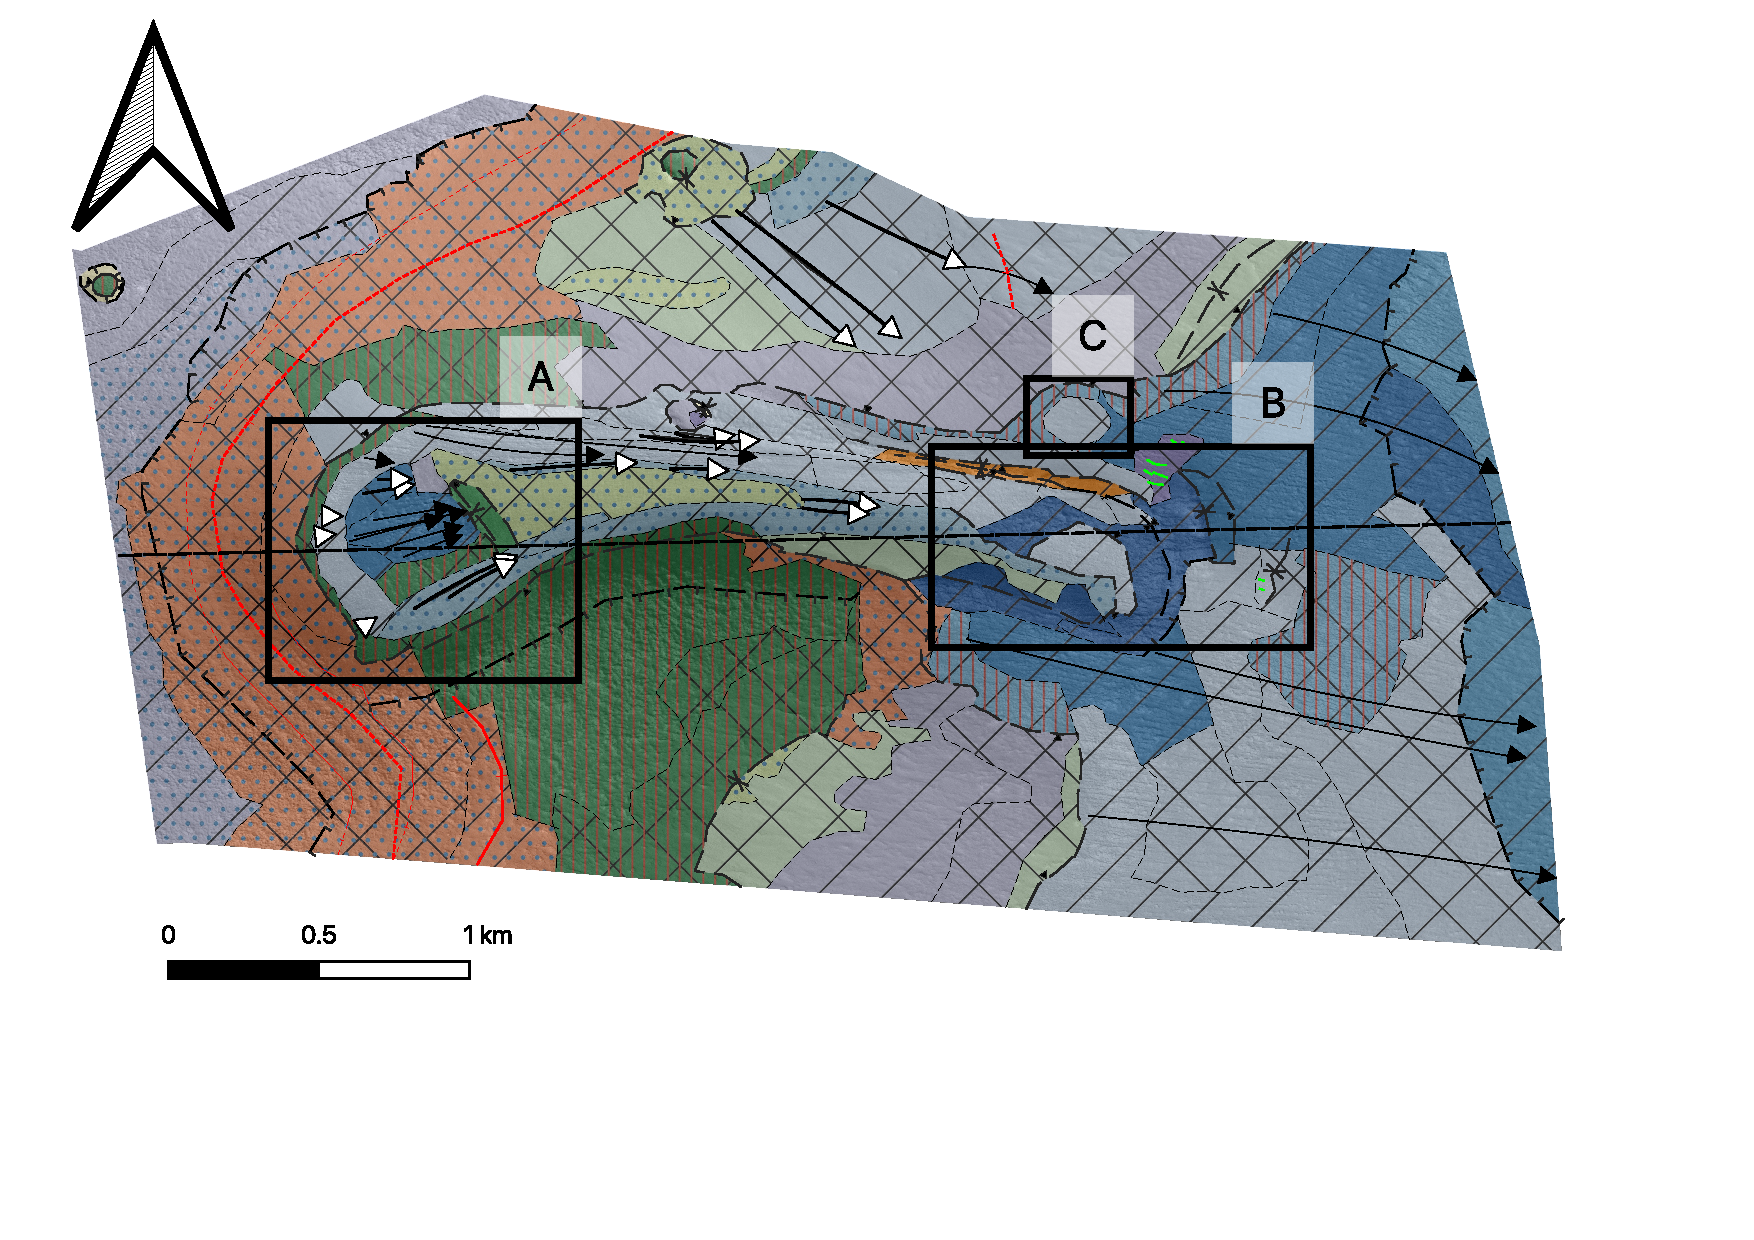
\includegraphics[
        width=\linewidth,
        height=0.65\textheight,
        keepaspectratio
    ]{Figures/Maps/HiRISE_Final_FigsMap.pdf}
    \label{fig:HiRISEFinal_a}
\end{subfigure}
\hfill
\begin{subfigure}{0.48\textwidth}
    \centering
    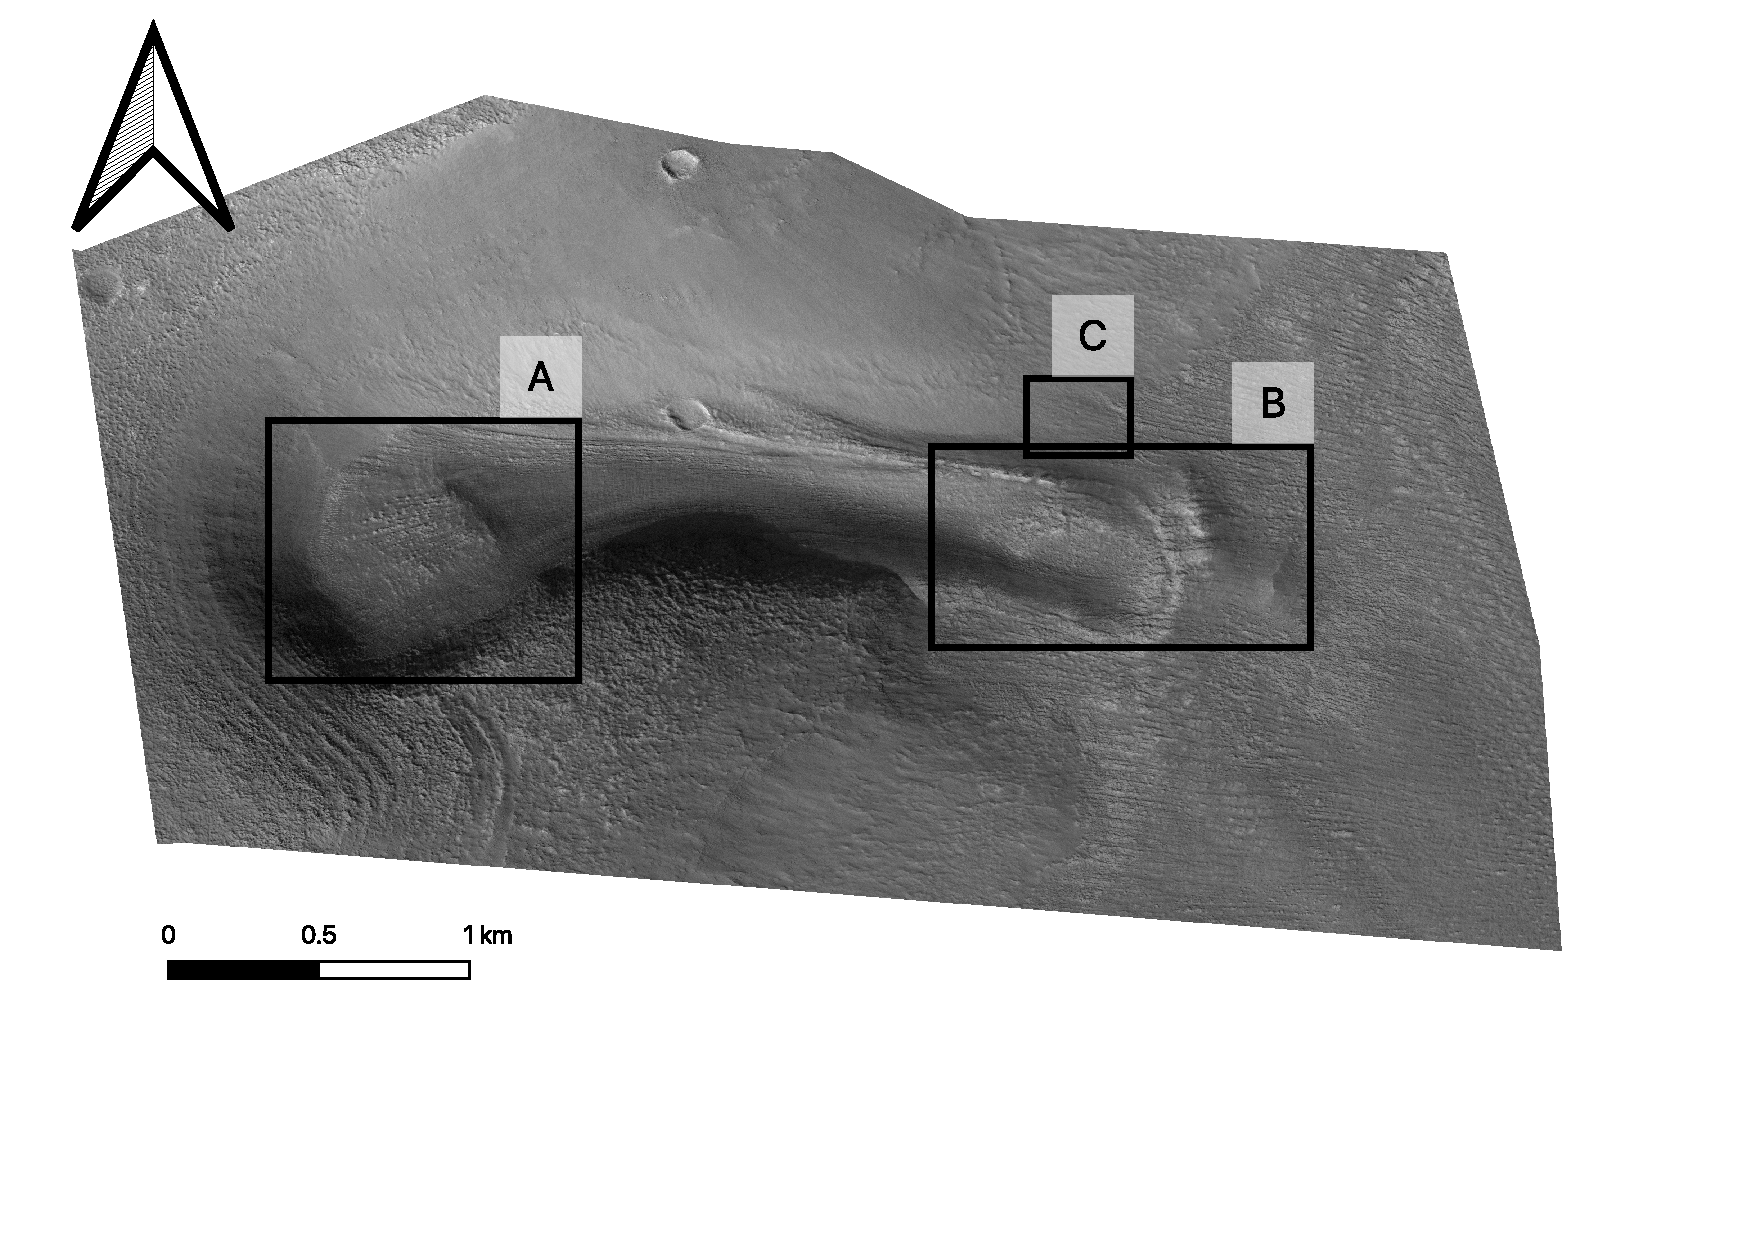
\includegraphics[
        width=\linewidth,
        height=0.65\textheight,
        keepaspectratio
    ]{Figures/Maps/HiRISE_Final_FigsImg.pdf}
    \label{fig:HiRISEFinal_b}
\end{subfigure}

\caption{Overview of alcove feature in NW Ismenius Cavus, mapped using HiRISE data. Inserts are highlighted (to be shown in alphabetical order).}
\label{fig:HiRISEFinal}

\end{figure}

\end{frame}
